\documentclass{article}
\usepackage{xcolor}
\usepackage{lipsum}
\usepackage{amsmath}
\usepackage{empheq}
\usepackage{indentfirst}
\setlength{\parindent}{2em}
\usepackage{amssymb}
\usepackage[UTF8]{ctex}
\usepackage{algorithm}
\usepackage{algorithmicx}
\usepackage{algpseudocode}
\usepackage{graphicx}
\usepackage{color}
\usepackage{tikz}
\author{My Name}
\title{The Title}
\begin{document}
	\section{abstract}
	distributed online learning,
	each learner optimizes its own learning parameter based on local data source and correspond with neighbours timely.
	
	privacy breaches(隐私泄露)
	
	centralized approach
	
	online data collection is inherently decentralized: data source are often widely distributed in different geographical locations.
	
	wide distribution:online learning
	high velocity:
	high dimensionality: sparse, spark and parallelize
	privacy concern: 
	
	exchange intermediate parameters with a random part of their own neighboring(spark trees: find a leaf and route to the corresponding sub-tree)
	
	distributed online learning
	
	similar to the mini-batch online learning. each iteration, the process receives K instances. Then each node processes one of the instances and updates its local model.
	These nodes communicate with each other to keep the consistency of their local model.
	
	A key factor in designing a distributed algorithm is the communication load between nodes.
	
	\section{INTRODUCTION}
	All nodes exchange their local parameter with their neighboring nodes.
	
	{\color{purple} For the privacy mechanism, differentially private framework is proposed with sensitive data}
	
	high-dimensional. 
	
	sparse solution.
	
%	\begin{tikzpicture}[sibling distance=10em,
%  every node/.style = {shape=rectangle, rounded corners,
%    draw, align=center,
%    top color=white, bottom color=blue!20}]]
%  \node {Sparse solution}
%    child { node {single-line} }
%    child { node {multi-line}
%      child { node {aligned at}
%        child { node {relation sign} }
%        child { node {several places} }
%        child { node {center} } }
%      child { node {first left,\\centered,\\last right} } };
%\end{tikzpicture}


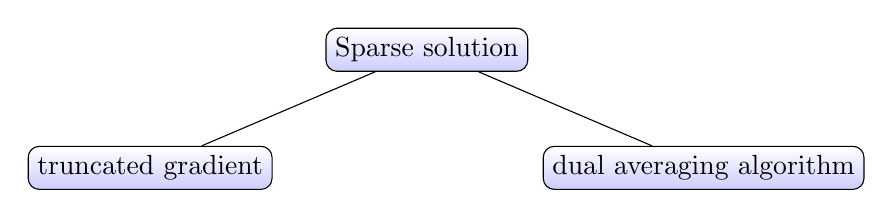
\begin{tikzpicture}[sibling distance=20em,
  every node/.style = {shape=rectangle, rounded corners,
    draw, align=center,
    top color=white, bottom color=blue!20}]]
  \node {Sparse solution}
    child { node {truncated gradient} }
    child { node {dual averaging algorithm}
       } ;
\end{tikzpicture}

DOLA take online mirror descent and $Lasso-L_1$ norm.

\section{EXPERIMENTS}
	\textbf{step 1} regard one CPU as one node. and equally distribute the dataset to the m nodes.
	
	There are three different topologies.
	
	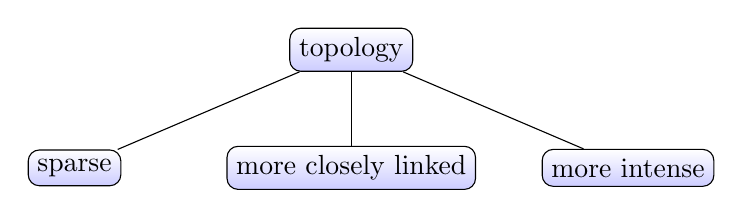
\begin{tikzpicture}[sibling distance=10em,
  every node/.style = {shape=rectangle, rounded corners,
    draw, align=center,
    top color=white, bottom color=blue!20}]]
  \node {topology}
    child { node {sparse} }
    child { node {more closely linked}}
    child { node {more intense}}
        ;
\end{tikzpicture}
	
\textbf{step 2}, communication matrix $A_t$. A map for communication.

\textbf{step 3},	
	
	openMPI
	
\section{Related Work}
differentially private centralized online learning.

\section{problem setting}
communication cost is not considered.

{\color{red} any node of the system can measure the regret of the whole system based on its local parameter}

use a time-variant matrix $A_t$ to conduct the communications among nodes.

Each node first gets the exchanged parameters and computes the weighted average of them, then updates the parameter $w_t^i$, finally broadcasts new parameter to its neighbours.

\begin{eqnarray*}
	\mathcal{G}_i(t) = \{(i,j):a_{ij}(t)>0\}.
\end{eqnarray*}

\subsection{Differential Privacy Model}
\textbf{Definition 2}
Let $\mathcal{A}$ denote differentially private DOLA.
Let $\mathcal{X}=<x_1^i, x_2^i,..., x_T^i>$ be a sequence of questions taken from an arbitrary node's loocal data source. Let $\mathcal{W}=<w_1^i, w_2^i, ..., w_T^i>$ be a sequence of T outputs of the node and $\mathcal{W} = \mathcal{A}(\mathcal{X})$. Then, our algorithm $\mathcal{A}$ is $\epsilon-$differentially private if given any adjacent question sequnces $\mathcal{X}$ and $\mathcal{X'}$ that differ in one question entry, the following holds:
\begin{eqnarray*}
	Pr[\mathcal{A} (\mathcal{X}) \in W] \leq e^{\epsilon}Pr[\mathcal{A} ( \mathcal{X}^{'} ) \in W ]
\end{eqnarray*}

	



		
	
	
	
	
\end{document}